\documentclass{article}
\usepackage{tikz}
\usepackage{geometry}
\geometry{a4paper, margin=1cm}

\begin{document}

% 左侧重构 (Left-side reconstruction)
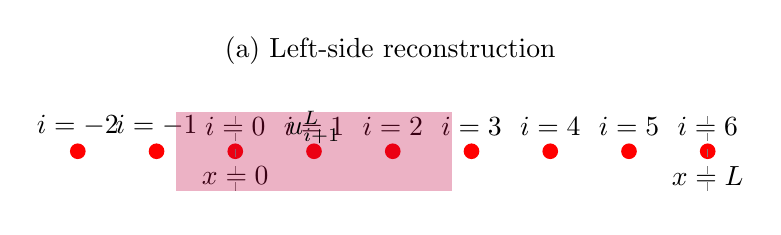
\begin{tikzpicture}
    % 设置坐标和样式
    \tikzset{
        dot/.style={circle, fill=red, inner sep=2pt},
        template/.style={rectangle, fill=purple, fill opacity=0.3, draw=none},
    }

    % 绘制网格点 (红点) 并命名节点
    \foreach \x in {-2,-1,0,1,2,3,4,5,6} {
        \node[dot] (p\x) at (\x,0) {};
        \node[above=2pt] at (\x,0) {\(i=\x\)};
    }

    % 绘制虚线 (x=0 和 x=L)
    \draw[dashed, gray] (0,-0.5) -- (0,0.5);
    \draw[dashed, gray] (6,-0.5) -- (6,0.5);
    \node[below=2pt] at (0,0) {\(x=0\)};
    \node[below=2pt] at (6,0) {\(x=L\)};

    % 绘制紫色模板 (从 i-1 到 i+2, 覆盖 i+1)
    \node[template, minimum width=3.5cm, minimum height=1cm] at (1,0) {};
    \node at (1,0.3) {\(u_{i+1}^L\)};

    % 设置标题
    \node[above=10pt] at (current bounding box.north) {(a) Left-side reconstruction};
    
    % 隐藏坐标轴
    \path[use as bounding box] (-2.5,-0.7) rectangle (6.5,0.7);
\end{tikzpicture}

% 右侧重构 (Right-side reconstruction)
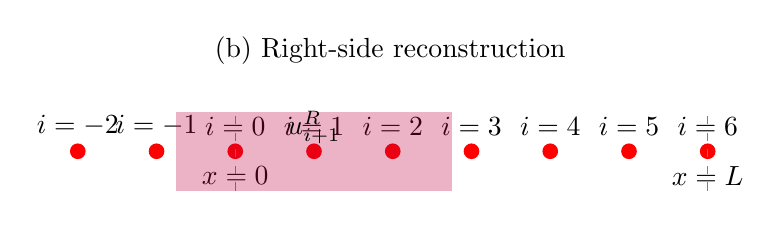
\begin{tikzpicture}
    % 设置坐标和样式
    \tikzset{
        dot/.style={circle, fill=red, inner sep=2pt},
        template/.style={rectangle, fill=purple, fill opacity=0.3, draw=none},
    }

    % 绘制网格点 (红点) 并命名节点
    \foreach \x in {-2,-1,0,1,2,3,4,5,6} {
        \node[dot] (p\x) at (\x,0) {};
        \node[above=2pt] at (\x,0) {\(i=\x\)};
    }

    % 绘制虚线 (x=0 和 x=L)
    \draw[dashed, gray] (0,-0.5) -- (0,0.5);
    \draw[dashed, gray] (6,-0.5) -- (6,0.5);
    \node[below=2pt] at (0,0) {\(x=0\)};
    \node[below=2pt] at (6,0) {\(x=L\)};

    % 绘制紫色模板 (从 i-1 到 i+2, 覆盖 i+1)
    \node[template, minimum width=3.5cm, minimum height=1cm] at (1,0) {};
    \node at (1,0.3) {\(u_{i+1}^R\)};

    % 设置标题
    \node[above=10pt] at (current bounding box.north) {(b) Right-side reconstruction};
    
    % 隐藏坐标轴
    \path[use as bounding box] (-2.5,-0.7) rectangle (6.5,0.7);
\end{tikzpicture}

\end{document}